%%%%%%%%%%%%%%%%%%%%%%%%%%%%%%%%%%%%%%%%%
% FRI Data Science_report LaTeX Template
% Version 1.0 (28/1/2020)
%
% Jure Demšar (jure.demsar@fri.uni-lj.si)
%%%%%%%%%%%%%%%%%%%%%%%%%%%%%%%%%%%%%%%%%

%----------------------------------------------------------------------------------------
%   PACKAGES AND OTHER DOCUMENT CONFIGURATIONS
%----------------------------------------------------------------------------------------
\documentclass[fleqn,moreauthors,10pt]{ds_report}
\usepackage[english]{babel}

\graphicspath{{fig/}}

%----------------------------------------------------------------------------------------
%   ARTICLE INFORMATION
%----------------------------------------------------------------------------------------

\JournalInfo{Machine Learning for Data Science 1, 2025-2026}
\Archive{Homework 4 Report}
\PaperTitle{Artificial Neural Networks}
\Authors{Denis Nedić}
\affiliation{\textit{dn98183@student.uni-lj.si}}

%----------------------------------------------------------------------------------------

\makeatletter
\renewcommand{\@maketitle}{%
\twocolumn[{%
\thispagestyle{empty}%
{
\includegraphics[height=2cm]{logo}}
\vskip-74pt%
{\raggedleft\small\sffamily\bfseries\@JournalInfo\\\@Archive\par}%
\vskip64pt%
{\raggedright\color{color1}\fontfamily{cmss}\fontseries{bc}\fontshape{n}\fontsize{20}{25}\selectfont \@PaperTitle\par}%
\vskip10pt%
{\raggedright\color{color1}\sffamily\fontsize{12}{16}\selectfont  \@Authors\par}%
\vskip8pt%
\begingroup%
\raggedright\sffamily\small%
\footnotesize\@affiliation\par%
\endgroup%
\vskip10pt%
}]%
}
\makeatother

\begin{document}

\flushbottom
\maketitle
\thispagestyle{empty}

%----------------------------------------------------------------------------------------
%   ARTICLE CONTENTS
%----------------------------------------------------------------------------------------

\section*{Introduction}
In Part 1 of this assignment, I implemented a fully-connected multi-layer artificial
neural network (ANN) for classification from scratch using only \texttt{NumPy},
with hand-written backpropagation and mini-batch SGD with momentum. I verified the
gradient implementation numerically and demonstrated that the network can perfectly
fit two non-linearly separable datasets.
\vspace{0.2cm}
\\
In Part 2, I re-implemented the same architecture in PyTorch and compared both
implementations across grid search accuracy, loss convergence, and training time.

%------------------------------------------------

\section*{Part 1: Custom ANN Implementation}

\textbf{1. Architecture}\\
The network is built around a \texttt{BaseANN} class with two subclasses:
\texttt{ANNClassification} and \texttt{ANNRegression}. It accepts an arbitrary list
of hidden layer sizes, per-layer activation functions (sigmoid or ReLU), an optional
L2 regularisation strength, and standard SGD hyperparameters. Weights are initialised
with Glorot uniform initialisation and biases are set to zero. The forward pass caches
all intermediate activations, which are reused during backpropagation.
\vspace{0.3cm}
\\
\textbf{2. Backpropagation}\\
Gradients are computed analytically using the chain rule, starting from the output
layer and propagating backwards. For classification with a softmax output, the output
error signal simplifies to the difference between the predicted probabilities and the
one-hot targets. This signal is then passed back through each hidden layer: the error
is propagated through the weight matrix and multiplied element-wise by the derivative
of the layer's activation function. Weight gradients at each layer are computed as
the outer product of the incoming activations and the local error signal, averaged
over the batch. L2 regularisation adds a penalty proportional to the weight values
to each weight gradient, leaving biases unregularised. The same backprop logic handles
both classification and regression, since the MSE loss with a linear output produces
the same form of output error signal.
\vspace{0.3cm}
\\
\textbf{3. Optimisation}\\
Training uses mini-batch SGD with momentum: at each step a velocity term accumulates
a fraction (0.9 by default) of the previous update and subtracts the current gradient
scaled by the learning rate. The data is randomly shuffled each epoch and processed
in mini-batches.
\vspace{0.3cm}
\\
\textbf{4. Gradient Verification}\\
To confirm the backpropagation is correct, I compared the analytical gradients to
numerical gradients computed by perturbing each weight slightly and measuring the
change in loss (symmetric finite differences with $\varepsilon = 10^{-5}$). The
maximum relative error across all weights and biases on a random 12-sample,
4-feature, 3-class problem was $1.37 \times 10^{-7}$, well below the acceptance
threshold of $10^{-5}$. This confirms that the gradient computation and the cost
function are consistent.

%------------------------------------------------

\section*{Part 2: Fitting the Datasets}

\textbf{Datasets.} Both datasets are two-dimensional and contain two classes.
\texttt{doughnut.tab} has 216 samples arranged in a concentric ring pattern, and
\texttt{squares.tab} has 400 samples arranged in a 2$\times$2 checkerboard pattern,
 four quadrants alternating between the two classes. Both are visualised in
Figure~\ref{fig:datasets}. Neither is linearly separable, so at least one hidden
layer is required in both cases.

\begin{figure}[h!]
    \centering
    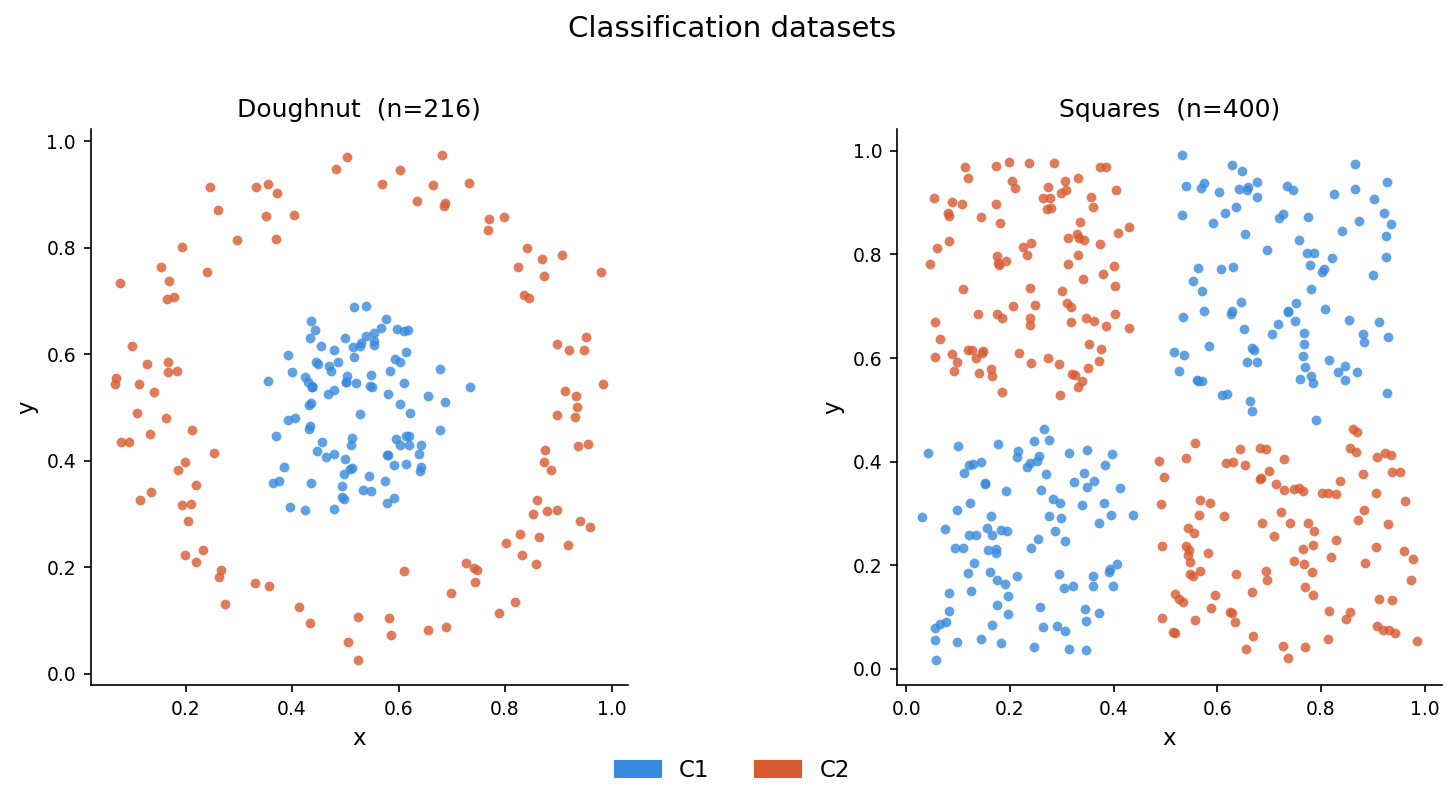
\includegraphics[width=\columnwidth]{datasets.png}
    \caption{Scatter plots of the two classification datasets. Each point is one
    sample; colour indicates the class label.}
    \label{fig:datasets}
\end{figure}
\vspace{0.3cm}

\textbf{Grid Search.} I searched over eight architectures (single hidden layers of size 3, 4, 6, and 8,
two-hidden-layer networks of size $[3,3]$, $[4,4]$, $[6,6]$, and a three-layer
$[4,4,4]$ network) with learning rates 0.1 and 0.3, evaluated over 5 random seeds
for 3000 epochs with full-batch training.
Table~\ref{tab:gridsearch} shows the smallest architecture that achieved 100\%
training accuracy across all seeds.

\begin{table}[h!]
    \centering
    \caption{Smallest architecture achieving 100\% mean accuracy across all 5 seeds.}
    \vspace{0.1cm}
    \label{tab:gridsearch}
    \resizebox{\columnwidth}{!}{%
    \begin{tabular}{llcc}
        \hline
        \textbf{Dataset} & \textbf{Model} & \textbf{Architecture} & \textbf{LR} \\
        \hline
        Doughnut & Custom  & {[3]}  & 0.3 \\
        Doughnut & PyTorch & {[3]}  & 0.3 \\
        Squares  & Custom  & {[6]}  & 0.3 \\
        Squares  & PyTorch & {[6]}  & 0.3 \\
        \hline
    \end{tabular}%
    }
    \vspace{0.1cm}
\end{table}

Both implementations agree on the minimal architecture. The doughnut problem only
needs 3 hidden neurons, while squares requires 6, reflecting the more complex
decision boundary of the checkerboard pattern. In both cases a learning rate of 0.3 was needed for reliable
convergence, for example at learning rate 0.1, some architectures stalled near random accuracy.

The three-hidden-layer architecture $[4,4,4]$ performed worst at LR~$= 0.1$,
achieving only around 52\% mean accuracy (near random) on both datasets. With
three stacked sigmoid layers and a small learning rate, gradient signals decay too
much before reaching the first layer. I suspect this has to do something with vanishing gradients.
\vspace{0.3cm}

\textbf{Training accuracy.} Both models achieve 100\% training accuracy on both
datasets with the minimal architectures found above. For these particular datasets,
this is a meaningful result. As visible in Figure~\ref{fig:datasets}, the class
boundaries are clean and noise-free since there are no overlapping points, no
mislabelled samples, and the two classes follow a clear geometric rule throughout
the entire dataset. Achieving 100\% training accuracy here means the network has
successfully learned the correct decision boundary, not that it has memorised
noise or overfit to quirks of a subset of the data.

%------------------------------------------------

\section*{Part 3: PyTorch Comparison}

\textbf{1. Implementation}\\
The PyTorch model uses the same architecture, initialisation scheme, and SGD with
momentum as the custom implementation. The key differences are in how the framework
handles the computation. Rather than manually stacking weight matrices and writing
the forward pass, layers are registered as named modules in a sequential container
and the forward pass is handled automatically. Instead of an explicit softmax in the
forward pass followed by a hand computed cross-entropy loss, PyTorch's built-in
cross-entropy loss function fuses both steps internally and operates on raw logits,
which is numerically more stable. Gradients are computed via automatic differentiation
rather than the hand derived chain rule, and parameter updates are handled by the
optimiser object instead of creating a manual velocity loop.
\vspace{0.3cm}
 
\textbf{2. Grid Search}\\
Both implementations agree completely on the best architecture for each dataset
(Table~\ref{tab:gridsearch}). The same failure patterns appear at low learning rates
and in deep architectures, which is expected given the identical initialisation and
optimiser settings. PyTorch shows slightly higher variance across seeds on some
intermediate architectures (e.g.\ $[3,3]$ on doughnut: 78.1\% vs.\ 80.0\% mean
accuracy), caused by differences in how the two implementations shuffle batches.
The internal random state is not shared, so even at the same seed the batch order
differs slightly.
\vspace{0.3cm}
 
\textbf{3. Loss Convergence}\\
Table~\ref{tab:convergence} compares training loss at selected epochs on the
doughnut dataset (architecture $[3]$, LR~$= 0.3$, single seed) across both
implementations and both batch sizes.

\begin{table}[h!]
    \centering
    \caption{Training loss vs.\ epoch (Doughnut, arch=[3], LR=0.3).}
    \vspace{0.1cm}
    \label{tab:convergence}
    \resizebox{\columnwidth}{!}{%
    \begin{tabular}{rcccc}
        \hline
        \textbf{Epoch} & \textbf{Cust-Full} & \textbf{Cust-Mini} & \textbf{Torch-Full} & \textbf{Torch-Mini} \\
        \hline
        1    & 0.7024 & 0.6944 & 0.7181 & 0.7352 \\
        334  & 0.3801 & 0.0048 & 0.6913 & 0.0071 \\
        667  & 0.0413 & 0.0023 & 0.6514 & 0.0028 \\
        1000 & 0.0159 & 0.0015 & 0.3015 & 0.0016 \\
        1333 & 0.0106 & 0.0011 & 0.0521 & 0.0011 \\
        3000 & 0.0044 & 0.0004 & 0.0056 & 0.0004 \\
        \hline
    \end{tabular}%
    }
    \vspace{0.1cm}
\end{table}

The most striking result is the difference between full-batch and mini-batch
training. With batch size 32, both implementations converge roughly ten times
faster per epoch and reach a final loss around ten times lower than their
full-batch counterparts. This is because with batch size 32 the weights are updated
7 times per epoch instead of once, so by epoch 334 the mini-batch models
have already performed over 2300 weight updates while full-batch has done only 334.
\\
Within each batch size variant, custom and PyTorch converge to virtually
identical final losses. The small remaining gap in full-batch is due to
the two implementations using different random number generators for weight
initialisation, so the same seed
produces different starting weights. With mini-batch the many small updates
average out this initialisation difference and both implementations converge
to essentially the same solution. The same pattern holds on squares.
\\
Interestingly, replacing sigmoid with ReLU across all hidden layers leads to
significantly worse convergence on these datasets. The full-batch ReLU network
stalls at a loss of around 0.27 after epoch 334 and makes no further progress,
while the mini-batch variant oscillates without consistently improving. Sigmoid
outperforms ReLU here, which is somewhat unexpected given ReLU's general popularity,
but makes sense in context: these are small, low-dimensional datasets with smooth
circular and quadrant boundaries, where sigmoid's smooth nonlinearity is better
suited than ReLU's piecewise-linear response.
\vspace{0.3cm}
\\
\\
\textbf{4. Training Time}\\
The custom NumPy implementation is substantially faster on these small datasets:
0.18\,s vs.\ 1.76\,s on doughnut and 0.28\,s vs.\ 2.94\,s on squares. On small
data with full-batch training, PyTorch's framework overhead dominates the actual
computation. Its speed advantage would emerge on larger datasets or with GPU
acceleration.


%------------------------------------------------

\section*{Conclusion}

Both the custom NumPy and PyTorch implementations successfully learn the decision
boundaries of the doughnut and checkerboard datasets, achieving 100\% training
accuracy with minimal architectures. 3 hidden neurons for doughnut and 6 for
squares, both with learning rate 0.3. It means the network has correctly
captured the underlying geometric rule, not memorised noise.

The gradient check confirmed the correctness of the hand-written backpropagation
with a maximum relative error of $1.37 \times 10^{-7}$. The two implementations
are algorithmically equivalent. Within each batch size variant they converge to
virtually identical final losses. Any remaining gap in full-batch runs is explained
by the two frameworks using different random number generators, meaning the same seed produces different initial weights
and therefore slightly different gradient trajectories.

The most practically relevant finding is the effect of batch size. Mini-batch
training with batch size 32 converges roughly ten times faster per epoch and
reaches a ten times lower final loss compared to full-batch, because the weights
are updated 7 times per epoch instead of once. With mini-batches the initialisation
difference between implementations also vanishes, since the many small updates
average it out. On small datasets like these, the custom NumPy implementation is
also considerably faster in wall-clock time than PyTorch due to framework overhead,
though this advantage would reverse on larger data or with GPU acceleration.

\end{document}